\documentclass[12pt]{article}
\usepackage{graphics}
\usepackage[top=1in,bottom=1in,left=1in,right=1in]{geometry}
\usepackage{alltt}
\usepackage{array}	
\usepackage{graphicx}
\usepackage{tabularx}
\usepackage{verbatim}
\usepackage{setspace}
\usepackage{listings}

\usepackage{amssymb,amsmath, amsthm}
\usepackage{zed-csp}
\usepackage[cc]{titlepic}

\title{COMP 335: Introduction to Theoretical Computer Science\\
\ \\
Assignment 3}
\author{Nathan Grenier}
\date{\today \\ Fall 2024}

\begin{document}
\begin{spacing}{1.5}
      \maketitle

      \newpage

      \begin{enumerate}

            \item[1.] [20 Points] For each of the following languages over $\Sigma = \{a,b\}$, write a regular grammar and then convert it into an equivalent NFA using the procedure described in class.

                  \begin{enumerate}
                        \item[(a)] (10 Points) $L(r) \text{ where } r= ((a+b)(a+b))^*b+a((a+b)(a+b))^*$

                              \textbf{G:}
                              \begin{itemize}
                                    \item $S \rightarrow A|B|\lambda$
                                    \item $A \rightarrow aD|bD$
                                    \item $D \rightarrow aD|bD|bS$
                                    \item $B \rightarrow aC$
                                    \item $C \rightarrow aaS|abS|baS|bbS|$
                              \end{itemize}

                              \textbf{Equivalent NFA of G:}

                              \begin{figure}[h!]
                                    \centering
                                    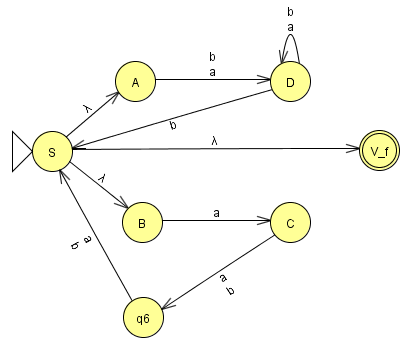
\includegraphics[width=0.65\textwidth]{img/q1/q1a(NFA).png}
                              \end{figure}
                              \newpage
                        \item[(b)] (10 Points) $\{w \in \{a,b\}^* : w \text{ ends in $a$ and $|w| \equiv 1$ } (\mod 3) \}$

                              \textbf{G:}
                              \begin{itemize}
                                    \item $S \rightarrow aA|bA|a$
                                    \item $A \rightarrow aB|bB$
                                    \item $B \rightarrow aS|bS$
                              \end{itemize}

                              \textbf{Equivalent NFA of G:}

                              \begin{figure}[h!]
                                    \centering
                                    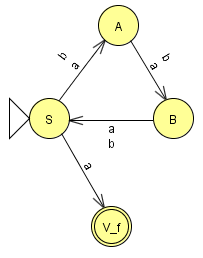
\includegraphics[width=0.35\textwidth]{img/q1/q1b(NFA).png}
                              \end{figure}

                  \end{enumerate}

                  \newpage
            \item[2.] [25 Points] Fix an alphabet $\Sigma$. For any string $w$ with $|w| \geq 2$, let $skip(w)$ be the string obtained by removing the first two symbols of $w$. Define 2 operators on languages:
                  $$f_1(L)=\{w \in \Sigma^* : skip(w) \in L \}$$
                  $$f_2(L)=\{skip(w) \in \Sigma^* : w \in L \}$$

                  \begin{enumerate}
                        \item[(a)] (5 Points) Consider $L' = L(bba^*)$ over tha alphabet $\Sigma = \{a,b \}$. Write a regular expression representing $f_1(L')$. Write another regular expression representing $f_2(L')$.
                              $$r_1 = (a+b)(a+b)bba^*$$
                              $$r_2 = a^*$$

                        \item[(b)] (10 Points) Claim: For every regular language $L$ the language $f_1(L)$ is regular. Clearly state whether the claim is TRUE or FALSE, and then prove your answer.

                              \textbf{Answer:} TRUE

                              \textbf{Proof:} Since $L$ is regular, there exists a DFA that accepts $L$. We define a new DFA $M'$ based on $M$, and will show that $L(M') = f_1(L(M))=f_1(L)$. This will show that $f_1(L)$ is regular.

                              We start by creating a DFA for L($bba?*$):
                              \begin{figure}[h!]
                                    \centering
                                    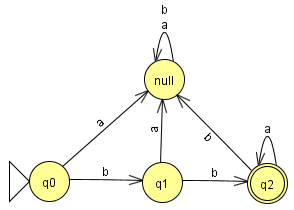
\includegraphics[width=0.45\textwidth]{img/q2/q2b(M).png}
                              \end{figure}
                              \newpage
                              Then, we create a new DFA $M'$ that accepts $f_1(L)$. We do this by adding states that accept any 2 characters from the alphabet $\Sigma$ at the start of the string in any word $w$:

                              \begin{figure}[h!]
                                    \centering
                                    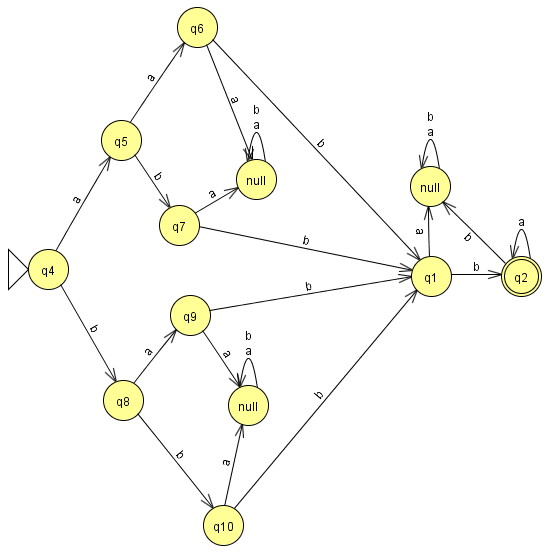
\includegraphics[width=0.6\textwidth]{img/q2/q2b(M').png}
                              \end{figure}

                              \newpage
                        \item[(c)] (10 Points) Claim: For every regular language $L$ the language $f_2(L)$ is regular. Clearly state whether the claim is TRUE or FALSE, and then prove your answer.

                              \textbf{Answer:} TRUE

                              \textbf{Proof:} Since $L$ is regular, there exists a DFA that accepts $L$. We define a new DFA $M'$ based on $M$, and will show that $L(M') = f_2(L(M))=f_2(L)$. This will show that $f_2(L)$ is regular.

                              We start by creating a DFA for L($bba^*$):
                              \begin{figure}[h!]
                                    \centering
                                    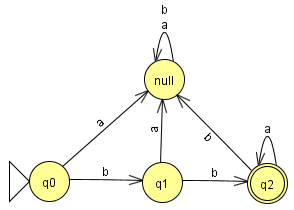
\includegraphics[width=0.45\textwidth]{img/q2/q2b(M).png}
                              \end{figure}

                              Then, we create a new DFA $M'$ that accepts $f_2(L)$. Our new DFA $M'$ will accept any string $w$ that has the first two characters removed from the start of the string. If there is a valid path from the start state $q_0$ to another state $q$ after reading any 2 characters, the state $q$ is a valid starting state. The new DFA $M'$ essentially starts from all states reachable after reading two symbols in $M$. After that, it follows the same transitions as $M$:

                              \begin{figure}[h!]
                                    \centering
                                    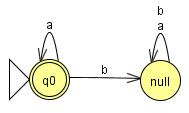
\includegraphics[width=0.3\textwidth]{img/q2/q2c(M').png}
                              \end{figure}
                  \end{enumerate}

                  \newpage
            \item[3.] [20 Points] For each of the following languages, use the Pumping Lemma and/or closure properties of regular languages to show that the language is not regular.

                  \begin{enumerate}
                        \item[(a)] (10 Points) $L_1=\{0^k1^l : k \geq l^4 \geq 0\}$

                              Mapping of potential values:
                              \begin{itemize}
                                    \item $l=0, k \geq 1$
                                    \item $l=1, k \geq 1$
                                    \item $l=2, k \geq 16$
                                    \item $l=3, k \geq 81$
                              \end{itemize}

                              Let $w=0^{m^4}1^m$ (i.e $l=m$, $k=m^4$).
                              \begin{itemize}
                                    \item Check: If $l=m$ and $k=m^4$ then $0^{m^4}1^m \in L$
                                    \item Check: $|w|=m^4 + m \geq m$
                              \end{itemize}

                              $$|m||m^4-m||m|$$
                              $$w=(00\dots 00)(00\dots 00)(11\dots 11)$$
                              $$|xy||z|$$

                              Therefore, $\exists j \geq 1, y=0^j$

                              When $i=0$: $w_0=0^{(m-j)+(m^4-m)}1^m = 0^{(m^4-j)}1^m $

                              \begin{itemize}
                                    \item $w_0 \in L_1 \text{ by PL}$
                                    \item $w_0 \not\in L_1 \text{ because } m^4-j < m^4 \therefore n_0(w_0) < n_1(w_0)^4 $
                              \end{itemize}

                              Therefore by contradiction, $L_1$ is not regular.
                              \newpage
                        \item[(b)] (10 Points) $L_2=\{a^n : n \text{ is not a perfect cube}\}$

                              Mapping of potential values:
                              \begin{itemize}
                                    \item $n=1^3=1$
                                    \item $n=2^3=8$
                                    \item $n=3^3=27$
                                    \item $n=4^3=64$
                              \end{itemize}

                              By the property of complements on regular languages, if $L_2$ is regular then $\overline{L_2}$ is also regular.

                              Let $w=a^{m^3}=(a^m)(a^{(m^3-m)})$. (i.e $n=m^3$).
                              \begin{itemize}
                                    \item Check: If $n=m^3$ then $a^{m^3} \in \overline{L_2}$
                                    \item Check: $|w|=m^3 \geq m$
                              \end{itemize}

                              $$|m||m^3-m|$$
                              $$w=(aa\dots aa)(aa\dots aa)$$
                              $$|xy||z|$$

                              Therefore, $\exists k \geq 1, y=a^k$

                              When $i=2$: $w_2=xyyz = a^ma^ka^{m^3-m}=a^{m^3+k} $

                              \begin{itemize}
                                    \item $w_2 \in \overline{L_2} \text{ by PL}$
                                    \item $w_2 \not\in \overline{L_2} \text{ because for } k \geq 1, \text{ not all strings } a^{m^3+k} \text{ are perfect cubes. } \\ \text{ In other words, } n_a(w_2) \neq m^3 \text{ for } m \geq 0$
                              \end{itemize}

                              Therefore by contradiction, $\overline{L_2}$ is not regular and $L_2$ is also not regular by association.
                  \end{enumerate}

      \end{enumerate}

\end{spacing}

\end{document}